\chapter{Documento dei Requisiti Software}
\label{cha:Documento dei Requisiti Software}

\begin{center} 
	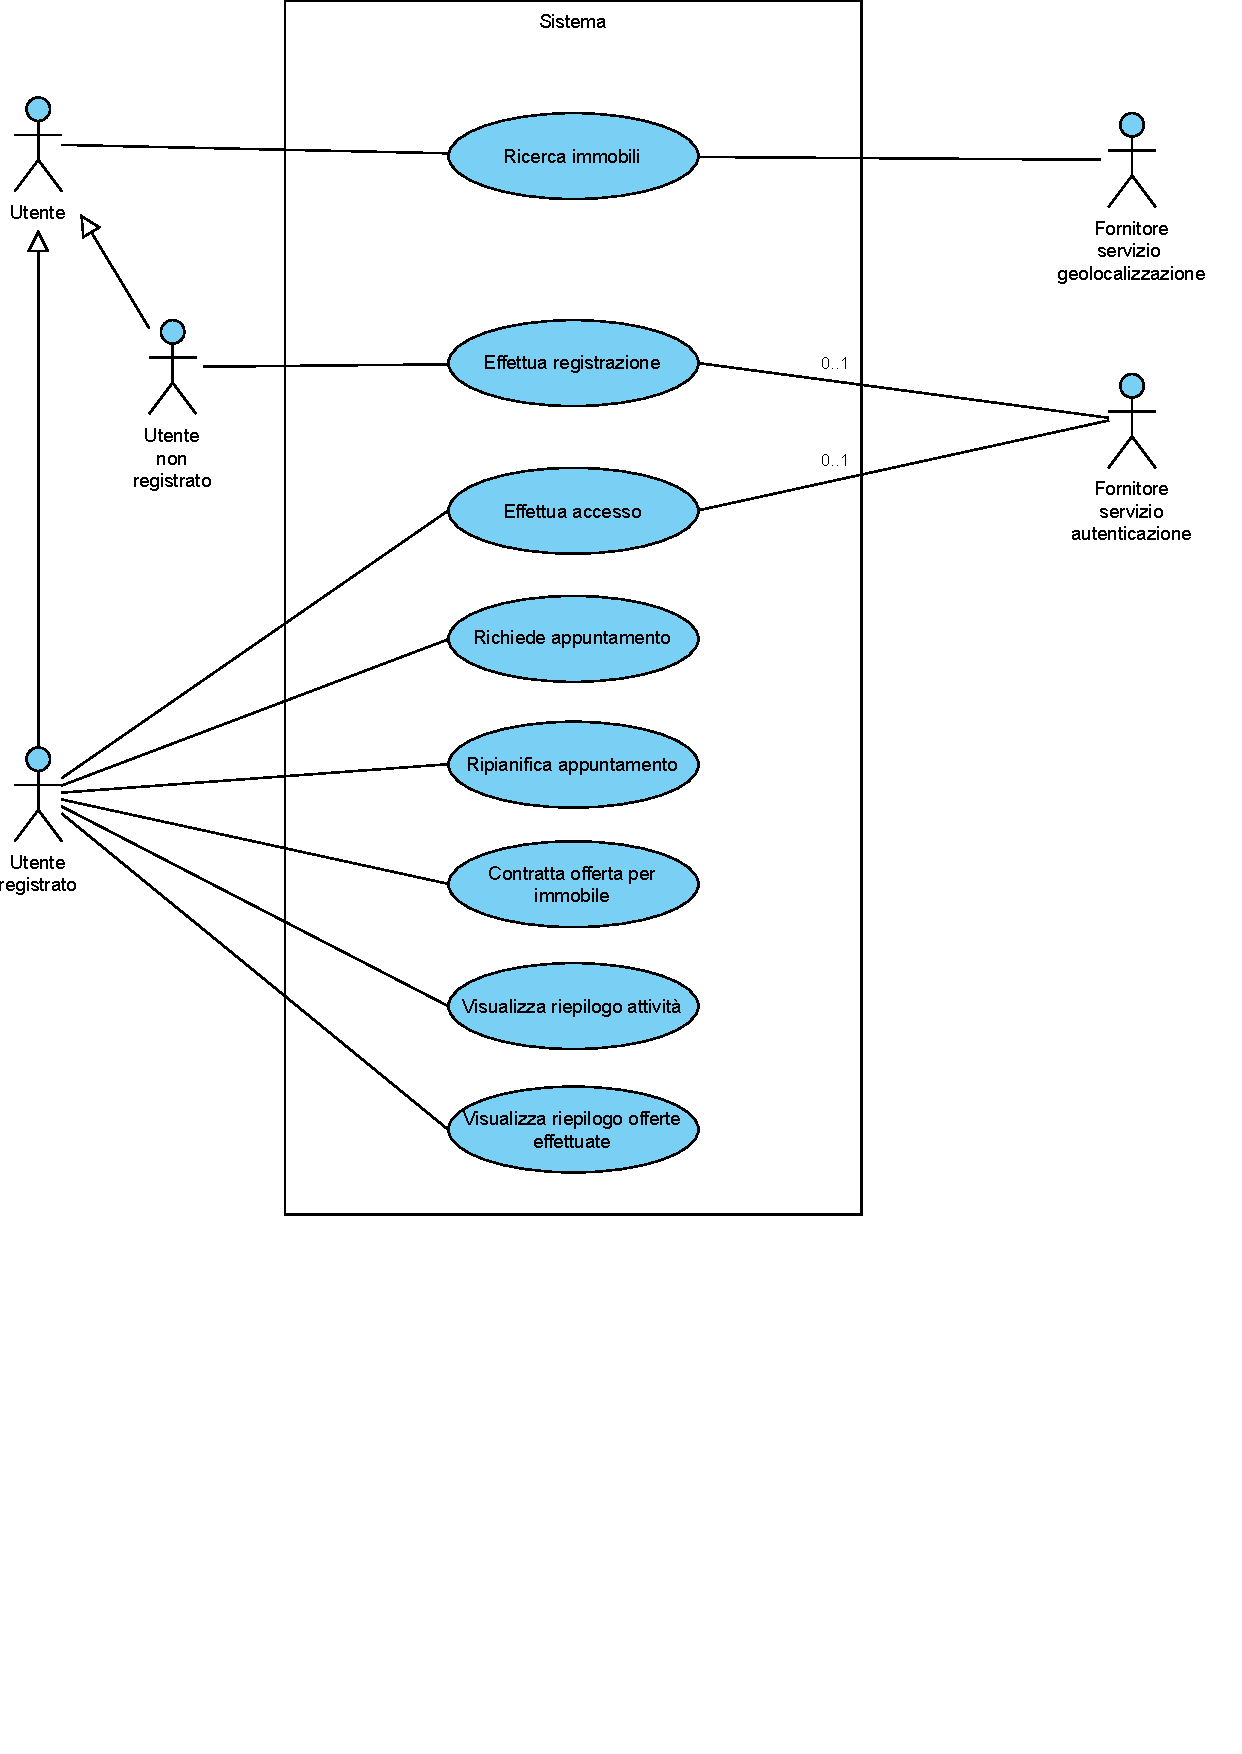
\includegraphics[width=0.9\textwidth]{UCDbusiness.pdf} 
\end{center}

\lipsum[1-4]

\customTable{c|X|Y}[Dizionario delle classi Prima Parte][tableTest]{\textbf{Classe} & \textbf{Descrizione} & \textbf{Attributi}}{
  AAA & BBB & CCC\\
  \hline
  \textbf{Account} & Generico utente che utilizza il sistema per effettuare ordini. & Test test test\\
}